%! TeX root = ../../main-en.tex
% 译自: chapters/zh/ch05.tex @ 5e07541:chapters/zh/ch05.tex
\chapter{Talking to the OS}
\label{chap:os}

By now you can write programs in C. You can use variables, make decisions and write loops, and you know what memory and pointers are. But there is one thing you may never have thought about: on its own, our program cannot actually do anything.

It cannot write on the screen by itself. It cannot read the keyboard by itself. It cannot open a file by itself. The screen, the keyboard and the disk all belong to the operating system (Section~\ref{sec:kernel-space}). If a program wants to do any of these things, it has to ask the operating system for help. Yet when we write programs, we never ``ask'' the operating system for anything. We just call functions like \texttt{printf}, \texttt{scanf} and \texttt{fopen}. Who wrote those functions? And how do they get hold of the operating system?

This chapter answers those two questions. The answer is two words: \emph{libraries} and \emph{system calls}.

The examples for this chapter are in the \texttt{code/en/ch05/} directory. Besides the Linux programs there are a few Windows programs. You can build them on Linux with the MinGW cross compiler (install \texttt{gcc-mingw-w64-x86-64} first) to get \texttt{.exe} files, and copy those to Windows to run them; in WSL you can also run them directly. To watch system calls we will also need a tool called \texttt{strace}.

\section{Libraries: Code in a Box}
\label{sec:library}

\subsection{Making Our Own Library}

A \emph{library} is a bundle of functions that have been written and compiled in advance and packed together for other programs to use. There is nothing mysterious about it; we can make one ourselves. First we write a header file that says which functions are in the library:

\codefile{code/en/ch05/greet.h}{The header file of the library}{lst:greet-h}

Then we write the functions themselves:

\codefile{code/en/ch05/greet.c}{The code of the library}{lst:greet-c}

We compile it into an object file and pack it into a library with the \texttt{ar} command:
\inputminted[linenos=false]{text}{code/en/ch05/out/build_lib.txt}

\texttt{ar} (short for archive) puts one or more object files into a ``parcel''. That parcel is a \emph{static library}.\lazynote{Static library}{At link time, the code you use is copied into your program. On Linux the name ends in \texttt{.a}.} By convention its name starts with \texttt{lib} and ends with \texttt{.a}. \texttt{ar t} lists what is in the parcel, and \texttt{nm} lists the functions in it: \texttt{T} means the function is right here (we saw this in Chapter~\ref{chap:hello}), and \texttt{U} means the function is used here but lives somewhere else. \texttt{greet} calls \texttt{printf}, but \texttt{printf} is not in our library. Our library is itself using someone else's library.

A program that uses this library only has to include the header file and call the functions in it:

\codefile{code/en/ch05/use_greet.c}{Using our own library}{lst:use-greet}

When compiling, we tell \texttt{gcc} where to look for libraries and which library to use:
\begin{minted}[linenos=false]{text}
gcc use_greet.c -L. -lgreet -o use_greet
\end{minted}
\texttt{-L.} means ``look for libraries in the current directory'', and \texttt{-lgreet} means ``use \texttt{libgreet.a}'' (you leave out the \texttt{lib} at the front and the \texttt{.a} at the end). The result:
\inputminted[linenos=false]{text}{code/en/ch05/out/use_greet.txt}

\texttt{use\_greet.c} has no idea how \texttt{greet} and \texttt{sum\_to} are written. It only read the header file, so it knows what the two functions are called, what arguments they want and what they give back. That is the whole point of a library: someone does a job well and wraps it up, and everyone else just picks it up and uses it, without caring how it works inside (Figure~\ref{fig:toolbox}).

\begin{figure}[htbp]
  \centering
  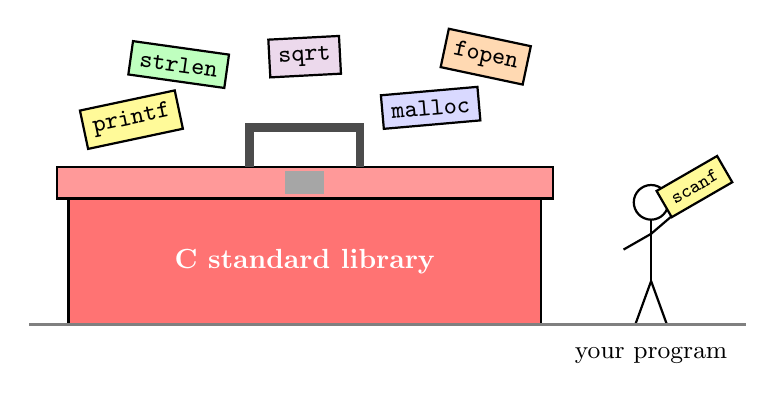
\begin{tikzpicture}[line width=0.8pt]
    % The toolbox
    \filldraw[fill=red!55] (0,0) rectangle (6,1.6);
    \filldraw[fill=red!40] (-0.15,1.6) rectangle (6.15,2.0);
    \draw[line width=3pt, gray!60!black] (2.3,2.0) -- (2.3,2.5) -- (3.7,2.5) -- (3.7,2.0);
    \fill[gray!70] (2.75,1.65) rectangle (3.25,1.95);
    \node[white, font=\bfseries] at (3,0.8) {C standard library};
    % The tools
    \node[draw, fill=yellow!40, rotate=12, font=\ttfamily\small] at (0.8,2.6) {printf};
    \node[draw, fill=green!25, rotate=-8, font=\ttfamily\small] at (1.4,3.3) {strlen};
    \node[draw, fill=blue!15, rotate=5, font=\ttfamily\small] at (4.6,2.75) {malloc};
    \node[draw, fill=orange!30, rotate=-12, font=\ttfamily\small] at (5.3,3.4) {fopen};
    \node[draw, fill=violet!15, rotate=3, font=\ttfamily\small] at (3.0,3.4) {sqrt};
    % A little person who has taken one
    \draw (7.4,1.55) circle (0.22);
    \draw (7.4,1.33) -- (7.4,0.55);
    \draw (7.4,0.55) -- (7.2,0) (7.4,0.55) -- (7.6,0);
    \draw (7.4,1.15) -- (7.05,0.95);
    \draw (7.4,1.15) -- (7.75,1.45);
    \node[draw, fill=yellow!40, rotate=30, font=\ttfamily\scriptsize] at (7.95,1.75) {scanf};
    \node[font=\small, align=center] at (7.4,-0.4) {your program};
    \draw[gray, line width=1pt] (-0.5,0) -- (8.6,0);
  \end{tikzpicture}
  \caption{A library is like a toolbox: the tools are ready-made, just take one and use it}
  \label{fig:toolbox}
\end{figure}

\paragraph{Static and dynamic libraries.}
When you link with a static library, the linker copies the parts of the library you use into your program, just as they are. The program gets a little bigger, but it no longer needs the library when it runs. The other kind is the \emph{dynamic library} (its name ends in \texttt{.so} on Linux; on Windows it is a \texttt{.dll}). At link time, the linker only notes down ``this program needs that library''; when the program runs, the dynamic linker loads the library into memory. The \texttt{libc.so.6} we saw with \texttt{ldd} in Chapter~\ref{chap:hello} is a dynamic library. Even when hundreds of programs are running at once, memory needs only one copy of \texttt{libc.so.6}, and they all share it. That is why a dynamic library is also called a \emph{shared library}.

\subsection{The C Standard Library}

So who wrote \texttt{printf}? The answer is: the C \emph{standard library}.\lazynote{C standard library}{A set of functions and header files defined by the C standard. Every C compiler has to provide them.} The C standard does not only define the grammar of the language; it also defines a set of functions that every C program can use, together with the header files that declare them (Table~\ref{tab:libc}). Every function we have used so far---\texttt{printf}, \texttt{scanf}, \texttt{malloc}, \texttt{free}, \texttt{fopen}---comes from the C standard library.

\begin{table}[htbp]
  \centering
  \caption{Commonly used header files of the C standard library}
  \label{tab:libc}
  \begin{tabular}{lll}
    \toprule
    Header & What it covers & Examples \\
    \midrule
    \texttt{stdio.h}  & input/output, files & \texttt{printf}, \texttt{scanf}, \texttt{fopen}, \texttt{fclose} \\
    \texttt{stdlib.h} & memory, misc.        & \texttt{malloc}, \texttt{free}, \texttt{rand}, \texttt{exit} \\
    \texttt{string.h} & strings              & \texttt{strlen}, \texttt{strcpy}, \texttt{memcpy} \\
    \texttt{math.h}   & maths                & \texttt{sqrt}, \texttt{sin}, \texttt{pow} \\
    \texttt{time.h}   & time                 & \texttt{time}, \texttt{clock} \\
    \bottomrule
  \end{tabular}
\end{table}

The standard only says \emph{what} these functions do, not \emph{how} they do it. On every operating system, someone has written them following the standard:
\begin{itemize}
  \item On Linux the most common one is the GNU C library, called \emph{glibc}. It is the \texttt{libc.so.6} we have been using all along. There is also the small and tidy musl, and Android phones use one called Bionic.
  \item On Windows the C standard library comes from Microsoft's C runtime library, for example the older \texttt{msvcrt.dll} and the newer UCRT (\texttt{ucrtbase.dll}).
\end{itemize}
Don't mix up glibc and \emph{GLib}.\lazynote{glibc and GLib}{glibc is the C standard library; GLib is GNOME's toolkit library. Similar names, different things.} GLib is a different library. It is the foundation of the GNOME desktop and the GTK graphical toolkit, and it provides fancier tools such as linked lists, hash tables and event loops. It is written in C itself and uses the functions glibc provides---another example of a library using a library.

\section{Everyone Asks the OS: System Calls}
\label{sec:syscall}

\subsection{Three Ways to Print a Line}

However clever the C standard library is, it is still just ordinary code. It runs in user mode, and it is not allowed to touch the screen either. In the end it, too, has to ask the operating system. The program below prints a line in each of three ways, each one closer to the operating system than the last:

\codefile{code/en/ch05/layers.c}{Three ways to print a line}{lst:layers}

\inputminted[linenos=false]{text}{code/en/ch05/out/layers.txt}

\begin{enumerate}
  \item \texttt{printf} is a C standard library function. It is the easiest to use, and it can turn numbers into text using formats like \texttt{\%d}.
  \item \texttt{write} is not in the C standard library. It is a function defined by the POSIX standard.\lazynote{POSIX}{A standard interface shared by Unix-like operating systems. It defines functions such as \texttt{write} and \texttt{open}.} POSIX is a standard that Linux, macOS and other systems of that family all follow, and it is one step closer to the operating system than the C standard. \texttt{write} just writes out a string of bytes exactly as they are; it does no format conversion.
  \item \texttt{syscall} makes a \emph{system call} directly: it tells the operating system ``I want service number such-and-such, and here are the arguments''. \texttt{SYS\_write} is the number of the ``write'' service; on x86-64 Linux it is 1.
\end{enumerate}

The \texttt{\#define \_DEFAULT\_SOURCE} at the top of the program tells glibc: besides the C standard library, I also want Linux-specific functions such as \texttt{syscall}.

\subsection{Peeking at System Calls with strace}

So what is the difference between these three ways, as far as the operating system can tell? \texttt{strace} can tell us.\lazyhint{No \texttt{strace} yet? In WSL, run \texttt{sudo apt install strace}.} It records every system call a program makes. Let us look at \texttt{write} calls only:
\begin{minted}[linenos=false]{text}
strace -e trace=write ./layers
\end{minted}
\inputminted[linenos=false]{text}{code/en/ch05/out/strace_layers.txt}

Three methods, and to the operating system they look exactly the same: each one is a single \texttt{write} system call that writes some bytes to file number 1 (standard output). The number after the equals sign is how many bytes were actually written. The last line says the program exited with exit status 0. \texttt{printf}, \texttt{write} and \texttt{syscall} are like a set of Russian dolls: one inside another, and when you open them all the way, the same system call is sitting in the middle (Figure~\ref{fig:matryoshka}).

\begin{figure}[htbp]
  \centering
  \begin{tikzpicture}[line width=0.8pt]
    \foreach \x/\s/\c/\d/\t in {0/1.0/red!55/red!60!black/printf, 3.0/0.78/orange!60/orange!60!black/write, 5.5/0.6/yellow!60/yellow!40!black/syscall} {
      \begin{scope}[shift={(\x,0)}, scale=\s]
        % Body
        \filldraw[fill=\c] (0,0) .. controls (-1.2,0) and (-1.2,1.6) .. (-0.75,2.0)
                           .. controls (-0.9,2.3) .. (-0.55,2.6)
                           arc[start angle=180, end angle=0, radius=0.55]
                           .. controls (0.9,2.3) .. (0.75,2.0)
                           .. controls (1.2,1.6) and (1.2,0) .. (0,0);
        % Face
        \filldraw[fill=yellow!10] (0,2.6) circle (0.38);
        \fill (-0.13,2.66) circle (0.04) (0.13,2.66) circle (0.04);
        \draw (-0.12,2.47) arc[start angle=200, end angle=340, radius=0.13];
        \fill[red!40] (-0.24,2.52) circle (0.06) (0.24,2.52) circle (0.06);
        % Flower
        \fill[white] (0,1.0) circle (0.3);
        \fill[\d] (0,1.0) circle (0.12);
      \end{scope}
      \node[font=\ttfamily] at (\x,-0.35) {\t};
    }
    \draw[-{Stealth}, thick] (1.1,1.2) -- (2.2,1.2);
    \draw[-{Stealth}, thick] (3.85,1.0) -- (4.85,1.0);
    \node[font=\small, align=center] at (2.75,3.75) {One inside another; open them all the way\\and it is the same \texttt{write} system call};
  \end{tikzpicture}
  \caption{\texttt{printf}, \texttt{write} and \texttt{syscall} are like a set of Russian dolls}
  \label{fig:matryoshka}
\end{figure}

\subsection{The Order Window of a Restaurant}

You can picture a system call as the order window of a restaurant (Figure~\ref{fig:restaurant}). The customer (your program) is not allowed to walk into the kitchen (the kernel) and cook. All they can do is write what they want on a slip of paper and pass it in through the window. The waiter (the library) is very helpful: you just say ``A cheeseburger, please'' (call \texttt{printf}), and he fills in the slip for you (prepares the number and the arguments of the system call), passes it through the window (makes the system call), and when the food is ready, brings it back to you (hands the result back to your program).

\begin{figure}[htbp]
  \centering
  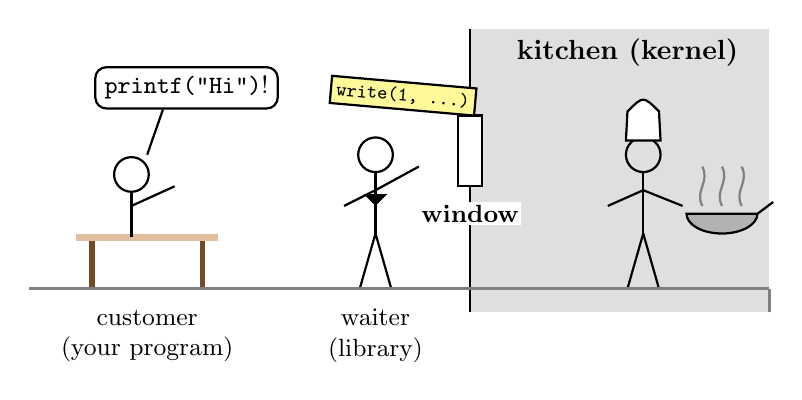
\begin{tikzpicture}[line width=0.8pt]
    % Kitchen wall and window
    \fill[gray!25] (5.6,0) rectangle (9.4,3.6);
    \draw (5.6,0) -- (5.6,3.6);
    \filldraw[fill=white] (5.45,1.6) rectangle (5.75,2.5);
    \node[font=\small\bfseries, fill=white, inner sep=1pt] at (5.6,1.25) {window};
    \node[font=\bfseries] at (7.6,3.3) {kitchen (kernel)};
    % The cook
    \draw (7.8,2.0) circle (0.22);
    \filldraw[fill=white] (7.58,2.18) -- (7.6,2.55) .. controls (7.8,2.75) .. (8.0,2.55) -- (8.02,2.18) -- cycle;
    \draw (7.8,1.78) -- (7.8,1.0);
    \draw (7.8,1.0) -- (7.6,0.3) (7.8,1.0) -- (8.0,0.3);
    \draw (7.8,1.55) -- (8.3,1.35);
    \draw (7.8,1.55) -- (7.35,1.35);
    % The pan
    \filldraw[fill=gray!60] (8.35,1.25) arc[start angle=180, end angle=360, x radius=0.45, y radius=0.25] -- cycle;
    \draw (9.25,1.25) -- (9.45,1.4);
    \foreach \x in {8.55,8.8,9.05} \draw[gray] (\x,1.35) .. controls (\x-0.1,1.55) and (\x+0.1,1.65) .. (\x,1.85);
    % The waiter
    \draw (4.4,2.0) circle (0.22);
    \draw (4.4,1.78) -- (4.4,1.0);
    \draw (4.4,1.0) -- (4.2,0.3) (4.4,1.0) -- (4.6,0.3);
    \draw (4.4,1.55) -- (4.95,1.85);
    \draw (4.4,1.55) -- (4.0,1.35);
    \fill[black] (4.25,1.5) -- (4.55,1.5) -- (4.4,1.35) -- cycle;
    \node[draw, fill=yellow!40, font=\ttfamily\scriptsize, inner sep=2pt, rotate=-5] at (4.75,2.75) {write(1, ...)};
    \node[font=\small, align=center] at (4.4,-0.3) {waiter\\(library)};
    % The customer and the table
    \fill[brown!50] (0.6,0.9) rectangle (2.4,1.0);
    \draw[brown!60!black, line width=2pt] (0.8,0.9) -- (0.8,0.3) (2.2,0.9) -- (2.2,0.3);
    \draw (1.3,1.75) circle (0.22);
    \draw (1.3,1.53) -- (1.3,0.95);
    \draw (1.3,1.35) -- (1.85,1.6);
    \node[draw, rounded corners, fill=white, font=\small] (say) at (2.0,2.85) {\texttt{printf("Hi")}!};
    \draw (say.south) ++(-0.3,0) -- (1.5,2.0);
    \node[font=\small, align=center] at (1.5,-0.3) {customer\\(your program)};
    \draw[gray, line width=1pt] (0,0.3) -- (9.4,0.3);
    \draw[gray, line width=1pt] (9.4,0) -- (9.4,0.3);
  \end{tikzpicture}
  \caption{A system call is like the order window of a restaurant}
  \label{fig:restaurant}
\end{figure}

\subsection{The Iceberg of Hello, world}

A Hello, world that prints just one line---how many times does it have to ask the operating system for help? Let us count with \texttt{strace -c} (\texttt{-c} stands for count):
\begin{minted}[linenos=false]{text}
strace -c ./hello
\end{minted}
The summary table is long, with one line for each kind of system call, so here we keep only the header and the total line at the end:
\inputminted[linenos=false]{text}{code/en/ch05/out/strace_hello_count.txt}

The \texttt{calls} column is the number of calls: 35 in total! (The \texttt{errors} column counts the calls that failed, for example looking for a file that does not exist.) Of all those, only the very last \texttt{write} actually prints the line:
\inputminted[linenos=false]{text}{code/en/ch05/out/strace_hello_tail.txt}

The other thirty-odd calls are all preparation done before \texttt{main} starts: the operating system runs the program (\texttt{execve}), the dynamic linker opens \texttt{libc.so.6} and maps it into memory (\texttt{openat}, \texttt{mmap}), sets up the memory permissions (\texttt{mprotect})\ldots{} All the things described in Section~\ref{sec:runtime} show up here, one by one. The final \texttt{exit\_group(0)} is the C standard library ending the whole program for us after \texttt{main} returns 0. The single \texttt{printf} line we wrote is just the tip of the iceberg (Figure~\ref{fig:iceberg}).

\begin{figure}[htbp]
  \centering
  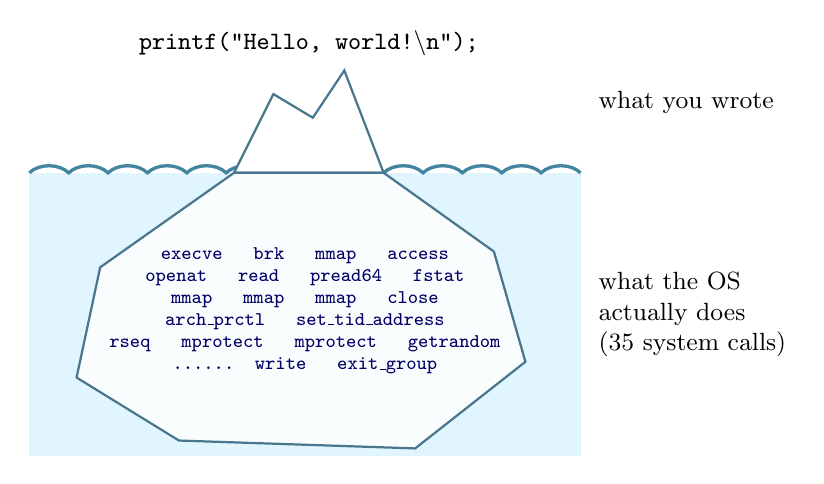
\begin{tikzpicture}[line width=0.8pt]
    \fill[cyan!12] (-3.5,-3.6) rectangle (3.5,0);
    \draw[cyan!60!black, line width=1.2pt]
      (-3.5,0) \foreach \k in {1,...,14} { .. controls ++(0.125,0.12) and ++(-0.125,0.12) .. ++(0.5,0) };
    % Above the water
    \filldraw[fill=white, draw=cyan!50!black] (-0.9,0) -- (-0.4,1.0) -- (0.1,0.7) -- (0.5,1.3) -- (1.0,0) -- cycle;
    \node[font=\ttfamily\small, fill=white, inner sep=1pt] at (0.05,1.65) {printf("Hello, world!\textbackslash n");};
    % Below the water
    \filldraw[fill=white, fill opacity=0.85, draw=cyan!50!black]
      (-0.9,0) -- (-2.6,-1.2) -- (-2.9,-2.6) -- (-1.6,-3.4) -- (1.4,-3.5) -- (2.8,-2.4) -- (2.4,-1.0) -- (1.0,0) -- cycle;
    \node[font=\ttfamily\scriptsize, align=center, text=blue!40!black] at (0,-1.75)
      {execve \quad brk \quad mmap \quad access \\ openat \quad read \quad pread64 \quad fstat \\
       mmap \quad mmap \quad mmap \quad close \\ arch\_prctl \quad set\_tid\_address \\
       rseq \quad mprotect \quad mprotect \quad getrandom \\ \ldots\ldots \quad write \quad exit\_group};
    \node[font=\small, anchor=west] at (3.6,0.9) {what you wrote};
    \node[font=\small, anchor=west, align=left] at (3.6,-1.8) {what the OS\\actually does\\(35 system calls)};
  \end{tikzpicture}
  \caption{The iceberg of Hello, world}
  \label{fig:iceberg}
\end{figure}

\subsection{What Is a System Call, Really?}

So how does the \texttt{syscall} function itself ``pass the slip through the window''? If we disassemble \texttt{syscall} in glibc, its core is just these few lines (x86-64):
\begin{minted}[linenos=false]{text}
mov    %rdi,%rax       # argument 1 (the call number) -> rax
mov    %rsi,%rdi       # the rest move along: rdi, rsi, rdx...
mov    %rdx,%rsi
mov    %rcx,%rdx
syscall                # into the kernel!
ret
\end{minted}
In the end, a system call is just one CPU instruction. On x86-64 it is called \texttt{syscall}; on RISC-V it is called \texttt{ecall}. Before executing it, the program puts the number of the service into an agreed register (\texttt{rax} on x86-64) and the arguments into a few other registers. When the instruction runs, the CPU switches from user mode to kernel mode and jumps to an entry point the kernel registered in advance (Section~\ref{sec:kernel-space}). The kernel looks at the number, sees what you want, does the job, puts the result in \texttt{rax}, then switches back to user mode and returns to the instruction right after \texttt{syscall}.

Linux provides more than three hundred system calls, and each has its own number. On x86-64, \texttt{write} is 1, \texttt{getpid} (``what is my process number?'') is 39, and \texttt{exit\_group} is 231. These numbers are listed in the header file \texttt{asm/unistd\_64.h}. Once a number is chosen it never changes, which is why a program compiled twenty years ago still runs on today's Linux.

\section{Writing a File}
\label{sec:file}

One more example. The program below creates a file and writes a sentence into it:

\codefile{code/en/ch05/file.c}{Writing a file}{lst:file}

\texttt{fopen} opens a file and gives back a \texttt{FILE *}---a pointer to some ``information about the file''. From then on, whenever you read or write this file, you hand that pointer to the standard library. \texttt{"w"} means you want to write: if the file does not exist it is created, and if it already exists it is emptied. \texttt{fprintf} is just like \texttt{printf}, except that it writes into the file instead of onto the screen. When you are done, \texttt{fclose} closes the file. If opening fails, \texttt{fopen} gives back \texttt{NULL}, so we check for that.

Let us use \texttt{strace} to see which system calls they turn into:\lazynote{File descriptor}{The number the kernel gives an open file. 0 is standard input, 1 is standard output, 2 is standard error.}
\begin{minted}[linenos=false]{text}
strace -e trace=openat,write,close ./file
\end{minted}
\inputminted[linenos=false]{text}{code/en/ch05/out/strace_file.txt}

\begin{table}[htbp]
  \begin{lazywide}
  \caption{C standard library functions and the system calls they use}
  \label{tab:file-syscalls}
  \begin{tabular}{lll}
    \toprule
    C standard library & Linux system call & What it does \\
    \midrule
    \texttt{fopen("diary.txt", "w")} & \texttt{openat} & open the file; the kernel returns 3 \\
    \texttt{fprintf(fp, ...)}         & \texttt{write(3, ...)} & write into file number 3 \\
    \texttt{fclose(fp)}               & \texttt{close(3)} & close file number 3 \\
    \bottomrule
  \end{tabular}
  \end{lazywide}
\end{table}

Compare with Table~\ref{tab:file-syscalls}: they match one to one. The kernel gives each open file a number, called a \emph{file descriptor}. 0 is standard input (the keyboard), 1 is standard output (the screen), 2 is standard error, and newly opened files are numbered from 3 on. When \texttt{printf} writes on the screen, it uses number 1; the 1 in \texttt{write(1, ...)} in \texttt{layers.c} means the same thing.

Notice that \texttt{fprintf} does not make a \texttt{write} straight away. It first saves up the text in a buffer and writes it all out in one go at \texttt{fclose}. A system call has to go into the kernel and back out again, which is much slower than an ordinary function call, so the standard library makes as few of them as it can---one more favour the waiter does for us.

\section{On \texorpdfstring{\NoCaseChange{Windows}}{Windows}: the \texorpdfstring{\NoCaseChange{Win32 API}}{Win32 API}}
\label{sec:win32}

\subsection{Writing Programs with the Win32 API}

Windows has its own kernel and its own system calls too, but Microsoft does not want programs to touch them directly. What Windows gives programmers is a different interface: the \emph{Win32 API}.\lazynote{API}{Application Programming Interface: the set of functions a system or a library offers to programs.} It consists of thousands of functions provided by a large group of dynamic libraries such as \texttt{kernel32.dll}, \texttt{user32.dll} and \texttt{gdi32.dll}. Opening files, creating windows, drawing, networking\ldots{} almost every program on Windows does its work through them.

First, here is a program that prints a line using the Win32 API:

\codefile{code/en/ch05/win_hello.c}{Printing a line with the Win32 API}{lst:win-hello}

\begin{itemize}
  \item \texttt{windows.h} is the main header file of the Win32 API.
  \item A \texttt{HANDLE} is a number Windows uses to refer to a ``thing'',\lazynote{Handle}{A number Windows uses to refer to a ``thing'' (a file, a window\ldots{}), rather like a file descriptor.} such as an open file or a window. It does much the same job as a file descriptor on Linux. \texttt{GetStdHandle(STD\_OUTPUT\_HANDLE)} gets the handle of standard output.
  \item \texttt{DWORD} is Windows' own name for a 32-bit unsigned integer type. The Win32 API is full of names like this, such as \texttt{BOOL} and \texttt{LPCSTR}. You get used to them after a while.
  \item \texttt{WriteFile} writes a string of bytes to a handle. Its last two arguments are for handing back how many bytes were actually written and for ``asynchronous'' reading and writing (which we don't need here, so we pass \texttt{NULL}). Notice that we pass it \texttt{\&written}---it has to write the result into our variable, so it needs the address (Section~\ref{sec:swap}).
\end{itemize}

Compile it on Linux with the MinGW cross compiler, and you get a Windows program:
\begin{minted}[linenos=false]{text}
x86_64-w64-mingw32-gcc win_hello.c -o win_hello.exe
\end{minted}
Copy \texttt{win\_hello.exe} to Windows and run it in a command prompt window (or just run \texttt{./win\_hello.exe} in WSL):
\inputminted[linenos=false]{text}{code/en/ch05/out/win_hello.txt}

Of course the Win32 API can do more than print text. The program below pops up a dialog box and asks you a question. The \texttt{MessageBoxW} it uses lives in \texttt{user32.dll}. (The \texttt{W} means the strings are made of ``wide'' characters, which can hold letters from almost any language, from Chinese to Greek; the \texttt{L} in front of each string means the same thing.)

\codefile{code/en/ch05/win_msgbox.c}{Popping up a dialog box}{lst:win-msgbox}

Double-click \texttt{win\_msgbox.exe} in Windows and a dialog box like the one in Figure~\ref{fig:msgbox} pops up.

\begin{figure}[htbp]
  \centering
  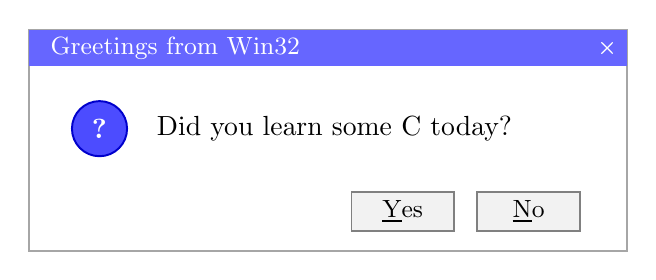
\begin{tikzpicture}[line width=0.7pt]
    \filldraw[fill=white, draw=gray!70] (0,0) rectangle (7.6,2.8);
    \fill[blue!60] (0,2.35) rectangle (7.6,2.8);
    \node[white, font=\small, anchor=west] at (0.15,2.575) {Greetings from Win32};
    \node[white, font=\small] at (7.35,2.575) {\texttimes};
    \filldraw[fill=blue!70, draw=blue!80!black] (0.9,1.55) circle (0.35);
    \node[white, font=\bfseries] at (0.9,1.55) {?};
    \node[anchor=west] at (1.5,1.55) {Did you learn some C today?};
    \filldraw[fill=gray!10, draw=gray] (4.1,0.25) rectangle (5.4,0.75);
    \node[font=\small] at (4.75,0.5) {\underline{Y}es};
    \filldraw[fill=gray!10, draw=gray] (5.7,0.25) rectangle (7.0,0.75);
    \node[font=\small] at (6.35,0.5) {\underline{N}o};
  \end{tikzpicture}
  \caption{The dialog box popped up by \texttt{win\_msgbox.exe} (a sketch)}
  \label{fig:msgbox}
\end{figure}

\subsection{printf on Windows}

Of course \texttt{printf} works on Windows too; it comes from the Windows C runtime library. \texttt{objdump -p} shows which functions each \texttt{.exe} imports from which DLLs (only the few we care about are listed here):
\inputminted[linenos=false]{text}{code/en/ch05/out/win_imports.txt}

\texttt{win\_printf.exe} imports \texttt{puts} from \texttt{msvcrt.dll}, not \texttt{printf}---the little optimization we met in Chapter~\ref{chap:hello} happens on Windows too (the code of \texttt{win\_printf.c} is in \texttt{code/en/ch05/}). And the \texttt{puts} in \texttt{msvcrt.dll} ends up calling none other than \texttt{WriteFile}.

\subsection{The Journey of WriteFile}

\texttt{WriteFile} is not the end of the road either. Inside Windows it still has several stops to make before it reaches the kernel. Below is real code, disassembled from the Windows system DLLs on this computer (with a different version of Windows, the addresses and details will differ):
\inputminted[linenos=false]{text}{code/en/ch05/out/win_chain.txt}

Let us go through it stop by stop:
\begin{enumerate}
  \item \texttt{WriteFile} in \texttt{kernel32.dll} is a single \texttt{jmp} instruction that jumps straight away. The real code moved to \texttt{KernelBase.dll} long ago; this is just a ``house number'' left behind so that old programs can still find it.
  \item \texttt{WriteFile} in \texttt{KernelBase.dll} checks the arguments and calls \texttt{NtWriteFile} in \texttt{ntdll.dll}. The address that \texttt{call} instruction goes to is ``the address of the next instruction, \texttt{0xb454d}, plus \texttt{0x1eb0bb}'', which is exactly \texttt{0x29f608}---the slot in the import table that holds the real address of \texttt{NtWriteFile}.
  \item \texttt{ntdll.dll} is the last stop in user mode. \texttt{NtWriteFile} puts the system call number 8 into \texttt{eax} and then executes \texttt{syscall} (older CPUs use \texttt{int 0x2e})---exactly like Linux, into the kernel it goes.
\end{enumerate}

Here is one big difference from Linux: the Windows system call numbers are not published, and they may change with every version of Windows. On this computer \texttt{NtWriteFile} is number 8; on another version of Windows it might be some other number. So programs on Windows never make system calls themselves. They always go through \texttt{ntdll.dll}, which ships together with Windows and fills in the right number. Linux, on the other hand, promises publicly that the numbers will never change, so programs can use them directly.

Figure~\ref{fig:stacks} puts the two systems side by side. The floors have different names, but the building has the same shape: the program calls a library, the library goes down floor by floor, and in the end a single \texttt{syscall} instruction walks into the kernel.

\begin{figure}[htbp]
  \begin{lazywide}
  \begin{tikzpicture}[
      layer/.style={draw, text width=54mm, minimum height=7.5mm, font=\footnotesize, align=center},
      line width=0.7pt,
    ]
    \foreach \x/\title/\a/\b/\c/\d in {
        0/Linux/{your program: \texttt{printf(...)}}/{C standard library glibc\\(\texttt{libc.so.6})}/{the \texttt{write} wrapper function}/{Linux kernel},
        6.6/Windows/{your program: \texttt{printf} or \texttt{WriteFile}}/{C runtime (\texttt{msvcrt.dll}), Win32 API\\(\texttt{kernel32.dll}, \texttt{KernelBase.dll})}/{\texttt{ntdll.dll}: \texttt{NtWriteFile}}/{Windows kernel (\texttt{ntoskrnl.exe})}} {
      \node[font=\bfseries] at (\x,4.1) {\title};
      \node[layer, fill=green!15]  at (\x,3.3) {\a};
      \node[layer, fill=yellow!20, minimum height=11mm] at (\x,2.2) {\b};
      \node[layer, fill=orange!20] at (\x,1.1) {\c};
      \node[layer, fill=gray!40, text=black] at (\x,-0.6) {\bfseries \d};
      \draw[red!70!black, line width=1.5pt, dashed] (\x-2.9,0.25) -- (\x+2.9,0.25);
      \draw[-{Stealth}, red!70!black, line width=1.2pt] (\x,0.75) -- (\x,-0.2);
      \node[red!70!black, font=\scriptsize\ttfamily, fill=white, inner sep=1pt] at (\x+0.65,0.25) {syscall};
    }
    \node[font=\scriptsize, anchor=east, red!70!black] at (-2.95,0.45) {user mode};
    \node[font=\scriptsize, anchor=east, red!70!black] at (-2.95,0.05) {kernel mode};
  \end{tikzpicture}
  \caption{Linux and Windows: the floors have different names, but the building has the same shape}
  \label{fig:stacks}
  \end{lazywide}
\end{figure}

\section{Back to the CPU}

Starting from \texttt{printf} and peeling away one layer after another, all that is left in the end is a single \texttt{syscall} instruction. That instruction makes the CPU switch from user mode to kernel mode and jump into the operating system's code.

This is a lot like the memory protection we met in Chapter~\ref{chap:memory}: neither of them is a software ``agreement''; both are built into the CPU hardware. The CPU has to remember which mode it is in. When it executes \texttt{syscall}, it has to save the address to come back to, switch modes and jump to the given entry point. And it has to stop a user program that steps out of bounds. Anyone who builds their own RISC-V CPU has to implement the \texttt{ecall} instruction by hand.

And a newly built CPU has no operating system, no glibc and no \texttt{printf}. To print a line on the screen, you either write bytes to the address of the serial port yourself (Section~\ref{sec:mmio}), or write a tiny ``kernel'' of your own to catch the \texttt{ecall}. Every layer we have seen in this chapter has to be built again from scratch. This book stops here; that road from scratch is a story for another time.

\section{Summary}

\begin{itemize}
  \item A library is a bundle of functions that have been written, compiled and packed together. The header file says what is in the library; the library holds the compiled code. A static library (\texttt{.a}) is copied into the program at link time; a dynamic library (\texttt{.so}, \texttt{.dll}) is loaded at run time and shared by everyone.
  \item The C standard library provides functions such as \texttt{printf}, \texttt{malloc} and \texttt{fopen}. On Linux it is usually glibc; on Windows it is Microsoft's C runtime library. GLib is a different library built on top of glibc.
  \item A program cannot operate the hardware by itself; it asks the operating system for help through system calls. Libraries wrap system calls, and in the end they all call them. \texttt{strace} shows every system call a program makes.
  \item A system call is a single CPU instruction (\texttt{syscall} on x86-64, \texttt{ecall} on RISC-V) that passes the number and the arguments in registers. Linux system call numbers are public and fixed.
  \item The kernel refers to open files by file descriptors (0, 1, 2, 3\ldots{}); Windows uses handles (\texttt{HANDLE}).
  \item Windows programs do their work through the Win32 API (\texttt{kernel32.dll}, \texttt{user32.dll} and so on), and in the end enter the kernel through \texttt{ntdll.dll}. Windows system call numbers are not published and change from version to version.
\end{itemize}

\lazysectionstar{Exercises}

\begin{enumerate}
  \item Add a new function \texttt{int max(int a, int b)} to \texttt{libgreet.a}, and call it from \texttt{use\_greet.c}. What do you need to change in the header file and in the library?
  \item Use \texttt{strace -c} to count the system calls made by the number-guessing game \texttt{guess} from Chapter~\ref{chap:c-basics}. Each time you make a guess, which kind of system call gets one more? (Hint: reading the keyboard.)
  \item In \texttt{file.c}, change \texttt{"w"} to \texttt{"a"} (append), and run the program three times. What is in \texttt{diary.txt}? Then use \texttt{strace} to see how the arguments of \texttt{openat} change.
  \item In \texttt{layers.c}, remove \texttt{fflush(stdout);}, then redirect the program's output to a file: \texttt{./layers > out.txt}. Open \texttt{out.txt}. Have the three lines changed order? Use \texttt{strace} to explain why.
  \item Using the Win32 API functions \texttt{CreateFileA}, \texttt{WriteFile} and \texttt{CloseHandle}, write a Windows version of \texttt{file.c}.
\end{enumerate}
